\chapter{Related Work}
\label{chapter:related_work}

The Steiner Multicycle Problem (\(\steinercycle\)) is related to vehicle routing problems, in particular to pickup and delivery problems. The literature for this class of problems is vast and considers multiple different restrictions and scenarios (\cite{surveyRouter}).

One of the most studied vehicle routing problems is the Travelling Salesman Problem, also known as TSP. In this problem we aim at finding the Hamiltonian cycle of least cost in a given complete graph. One of the most well known algorithms for the TSP is the Christofides Algorithm proposed by \cite{Christofides2022WorstCaseAO}. This algorithm produces a 3/2-approximation in metric graphs with the following process, as presented by \cite{williamsonApxAlgs}. Given a metric graph \(G\) we calculate its minimum spanning tree \(M\). Let \(O\) be the odd degree vertices in \(M\). By the handshaking lemma the are an even number of odd degree vertices in \(M\). One of the classic results in combinatorial optimization is that given a complete graph (on an even number of vertices) it is possible to calculate the perfect matching of minimum total cost in polynomial time, therefore we calculate the minimum cost perfect matching of \(O\). If we add the edges of \(O\) in \(M\) we create an Eulerian multigraph \(H\), since its connected and all vertices have even degree. Finally we can shortcut the duplicated edges to create a solution of no greater cost that corresponds to a Hamiltonian cycle.

As commented in Chapter \ref{chapter:introduction}, the TSP is related to the \(\steinercycle\), since an instance of one can be converted in polynomial time to an instance of the other. Given that, we proceed to present some relevant results in the literature for the \(\steinercycle\).

\cite{LINTZMAYER2020134} proposed a randomized PTAS for \(\steinercycle\) restricted to an Euclidean plane. The Euclidean \(\steinercycle\) consists in a set of terminals pairs distributed in a plane. That way, we aim at calculating the line segments that connects the points with the least cost, considering that the same line segment might be crossed more than once in the cost function.

% \cite{LINTZMAYER2020134} propuseram um PTAS aleatorizado para o \(\steinercycle\) restrito ao plano Euclidiano. O \(\steinercycle\) no caso Euclidiano consiste em um conjunto de pares de terminais distribuídos em um plano. Assim, desejamos calcular o conjunto de segmentos de reta de menor custo que conectam os terminais, levando em consideração que o comprimento de cada segmento de reta pode ser contabilizado múltiplas vezes na função de custo. Por exemplo, em um cenário em que temos apenas um par de terminais e uma solução em que um segmento de reta os conecta diretamente, o custo dessa solução seria duas vezes o comprimento da reta. Isso ocorre pois devemos contabilizar a ``ida'' e a “volta” do transporte que realiza as entregas entre os terminais.

% conferir a informacao desse paragrafo

In order to work in this problem, \cite{LINTZMAYER2020134} groups the terminal pairs in such a way that pairs that are far away from each other belongs to different groups. The authors give us guarantees that the union of the optimal solution calculated in each group is optimal in the general problem. Then, for each group of terminals pairs, we create a square called \textbf{root dissection square} which is a bounding box containing all terminals pairs of the group. This square has length of at most a constant times the cost of the optimal solution considering the terminals pairs in the square.

% A fim de tratar essa versão do \(\steinercycle\), \citeauthor{LINTZMAYER2020134} calculam agrupamentos de pares de terminais, em que pares de diferentes grupos estão distantes um do outro, de tal forma que a união da solução ótima de cada um dos grupos é a solução ótima para o problema geral. Na sequência, para cada agrupamento, é criado um quadrado, denominado \textbf{quadrado de dissecação raiz}, que contém todos os terminais do grupo. Esse partição é feita de tal forma que cada quadrado de dissecação raiz tem como comprimento máximo uma constante vezes o custo da solução ótima.

For each square we run a process of recursive dissection. In this process each square is subdivides into four squares of equal size, using a vertical and a horizontal lines. For each generated square during the partitioning, we select a limited number of points in its border as portals. That way the only valid solutions of the algorithm crosses the squares only through its portals. At the end of the process, each square that has not been partitioned is broken into cells, like in a grid. 

% Em seguida, cada quadrado de dissecação raiz é dividido em quatro sub-quadrados de mesma área usando linhas horizontais e verticais. Esse processo é realizado de maneira recursiva. Para cada quadrado gerado ao longo do particionamento, selecionamos um número limitado de pontos nas fronteiras dos quadrados como portais. Sendo assim, a solução do algoritmo atravessa as fronteiras do quadrados apenas pelos portais. Ao final do processo de divisão, cada ``quadrado folha'', o conjuntos dos menores quadrados gerados pelos cortes, é particionado em células, como em uma grade.

For each square \(R\), we define a memoization table \(M_R\), indexed by valid configurations of \(R\), in other words, subpartitions of the cells and portals of \(R\). Let \(\pi\) be a valid configuration of \(R\). then \(M_R(\pi)\) is the cost of the minimal solution that is compatible with \(\pi\) and conforms to \(R\). A solution is compatible with \(\pi\) when its lines segments respects the partition of \(\pi\). Besides that, a solution conforms with \(R\) when it is feasible, connects the necessary terminals pairs, only cross the borders in \(R\) through portals and makes that crossing a limited number of times.

% Para cada quadrado \textit{R}, definimos uma tabela de memoização \(M_R\) indexado por configurações válidas de \textit{R}, ou seja subpartições das células e portais de \textit{R}. Seja \(\pi\) uma configuração válida de \textit{R}. Temos que \(M_R(\pi)\) é o custo da menor solução compatível com \(\pi\) e que conforma com \textit{R}. Dizemos que uma solução é compatível com \(\pi\) quando os segmentos de reta da solução respeitam as partições de \(\pi\). Além disso, dizemos que uma solução conforma com \textit{R} quando ela é factível, conecta os pares de terminais necessários, somente atravessam a fronteira de \textit{R} nos portais e realiza essa travessia uma quantidade limitada de vezes.

To write an entry in \(M_R(\pi)\) we observe all possible configurations of the squares that where generated by subdividing \(R\), the ``children'' squares of \(R\). From all this configurations, we only consider the ones that are consistent with \(\pi\). Essentially, the authors show that the combined solutions of the four ``children'' squares generate a solution of that is compatible with \(\pi\) and conforms to \(R\).


(CITE PLACEHOLDER) presented a 3-approximation for \(\steinercycle\), considering metric and complete graphs. The algorithm was based on the work done by \cite{Christofides2022WorstCaseAO} for the metric TSP and consists of three basic steps.

The first step is to perform a 2-approximation for the Survivable Network Design Problem, considering a specific set of parameters, which will be detailed below. The authors described the Survivable Network Design Problem as follows: given a graph \(G\), a weight function \(w: E(G) \rightarrow Q+\), and a non-negative integer \(r_{ij}\) for each pair of vertices \(i\), \(j\) with \(i \neq j\), representing a connectivity requirement. The goal is to find a minimum weight subgraph \(G'\) of \(G\) such that, for every pair of vertices \(i, j \in V(G)\) with \(i \neq j\), there are at least \(r_{ij}\) edge-disjoint paths between \(i\) and \(j\) in \(G'\).

The authors also observed that from an \(\steinercycle\) instance it is easy to define a Survivable Network Design Problem instance by considering \(r_{ij} = 2\) for any vertices \(i\) and \(j\) that belong to the same terminal set and \(r_{ij} = 0\) otherwise. Those parameters are considered in the first step of the algorithm. In this way, it is possible to observe that the optimum value of the Survivable Network Design Problem is also a lower bound on the optimum for the Steiner Multicycle Problem: indeed an optimal solution for the Steiner Multicycle Problem is a feasible solution for the Survivable Network Design problem with the same cost.

Let \(T\) be a set of vertices of even size in a graph \(G\). A set \(J\) of edges in \(G\) is a \(T\)-join if the collection of vertices of \(G\) that are incident to an odd number of edges in \(J\) is exactly \(T\).

Let \(G'\) be the output of the 2-approximation, we consider \(T\) to be the set of odd degree vertices in \(G'\). Thus, the second step of the algorithm consists of calculating in polynomial time a minimum \(T\)-join \(J\) in \(G'\). Finally, as the third step, the final result is obtained by doubling the edges of \(J\) and by shortcutting an Eulerian tour for each component of H, to obtain a collection \(C\) of cycles in \(G\).

The \(\steinercycle\) was also studied in a more restricted variant, where we have a set of vertices as terminals and we must cover all terminals with only one cycle. This more restricted problem is known in the literature as Steiner Cycle Problem (SCP). It is possible to observe that the scenario in which all vertices are terminals the SCP is equivalent to the TSP.

% O \(\steinercycle\) também foi estudado na literatura em sua versão mais restrita, onde temos um subconjunto dos vértices como terminais e devemos cobri-los com um único ciclo. Essa versão mais restrita é conhecida na literatura como Problema do Ciclo de Steiner, ou do inglês Steiner Cycle Problem (SCP). É fácil observar que no caso de todos vértices serem terminais, o SCP é equivalente ao famoso Problema do Caixeiro Viajante, ou TSP.

The Steiner Cycle Problem (SCP) was proposed by \cite{SalazarSteinerCycle}. The authors analysed the polyhedral structured associated to the problem and introduced two lifting strategies to generate inequalities facet defining based on the TSP polytope.

% O Steiner Cycle Problem (SCP) for proposto por \cite{SalazarSteinerCycle} onde ele analisou a estrutural poliedral associada ao problema e introduziu duas estratégias de \textit{lifting} para gerar desigualdades definidoras de facetas baseadas no polítopo do TSP.

\cite{SteinovaSteinerCycle} presented a 3/2-approximation for the SCP in metric graphs. The authors also have shown that there is no approximation in constant time for general graphs, unless \(\poly = \nonpoly\). This result implies that the \(\steinercycle\) is \(\nonpolyopt\)-hard in general graphs.

% \cite{SteinovaSteinerCycle} apresentou uma 3/2-aproximação para o SCP em grafos métricos e demonstrou que não existe uma aproximação de tempo constante para o SCP em grafos gerais, a não ser que \(\poly = \nonpoly\). Desse resultado podemos inferir que o \(\steinercycle\) é NPO-difícil para grafos gerais.

Another problem related to the \(\steinercycle\) is the Steiner Forest Problem (SFP), where instead of using cycles to connect terminals pairs, we restrict ourselves to use only trees. In an equivalent way to the \(\steinercycle\) and SCP, the SFP generalizes the Steiner Tree Problem (STP). The STP is one of the most studied problems in the combinatorial optimization literature. The problem proposes to find the subgraph with minimum cost that connects a set of vertices in the graph. It was one of the \(\nonpoly\)-complete problems cited by \cite{Karp1972}.

% Outro problema relacionado ao \(\steinercycle\) é o Problema da Floresta de Steiner, ou da sigla em inglês SFP, onde ao invés de realizar as conexões entre pares de terminais usando ciclos, nos restringimos a usar apenas árvores. De maneira equivalente aos problemas \(\steinercycle\) e SCP, o SFP generaliza o Problema da Árvore de Steiner. O STP é um dos problemas mais estudados da literatura de otimização combinatória, nele desejamos conectar um subconjunto dos vértices com o subgrafo conexo de menor custo, que naturalmente implica em um subgrafo sem ciclos. Ele foi um dos problemas \(\nonpoly\)-completo citados por \cite{Karp1972}.

\cite{split-graphs} investigated the complexity of finding the minimum Steiner Tree in subclasses of split-graphs. It is known that the problem in \(\nonpoly\)-complete in general graphs. However, the authors have shown that the problem is treatable in polynomial time for tree-convex split-graphs, with convexity in the clique \(K\), although it still is \(\nonpoly\)-complete when the convexity is in the independent set \(I\).

% \cite{split-graphs} investigaram a complexidade de se encontrar a Árvore de Steiner mínima em subclasses de grafos-\textit{split}. Sabe-se que o problema é \(\nonpoly\)-completo em grafos-\textit{split} gerais. Os autores demonstraram que o problema passa a ser tratável em tempo polinomial para grafos-\textit{split} \textit{tree-convex} com convexidade na clique \(K\), apesar de permanecer \(\nonpoly\)-completo quando a convexidade é no conjunto independente \(I\).

\cite{KleinTSP} proposed a framework to obtain PTAS for multiple problems in planar graphs that consists in four steps. The first step creates an subgraph \(H\) called \textbf{spanner}. \(H\) has the spanning (there is a solution of cost \((1 + \epsilon) \opt\) in \(H\)) and shortness (the length of \(H\) is bounded by a constant times \(\opt\)) properties. The second step is to find a set of edges of \(H\) of cost at most \(\mathcal{O}(\epsilon \opt)\) and contract \(H\) on those edges. According to the results from \cite{Demaine2010}, the resultant graph of this process has bounded tree-width. The third step consists of using a dynamic programming approach in the bounded tree-width graph in order to obtain a optimal solution. Finally the solution is the union of the resulting graph from the DP with the set of edges that were contracted.

% \cite{KleinTSP} propôs um arcabouço, ou \textit{framework}, para se obter PTASes em grafos planares que consiste em quatro etapas. A primeira etapa procura gerar um subgrafo \(H\), denominado \textit{gerador}, com as propriedades de \textbf{geração} (existe uma solução de tamanho máxima \((1 + \epsilon) \opt\) em \(H\)) e \textbf{breviedade} (o comprimento de \(H\) é limitado por uma constante vezes \(\opt\)). A segunda etapa consiste em encontrar um conjunto de arestas de \(H\) de custo máximo \(\mathcal{O}(\epsilon \opt)\) e contrair \(H\) com esse conjunto de arestas. Segundo o resultado de \cite{Demaine2010}, o grafo gerado por esse processo possui uma decomposição em árvore com largura limitada. A terceira etapa consiste em aplicar uma estratégia de programação dinâmica no grafo de largura de árvore limitada a fim de obter uma solução aproximadamente ótima. Assim, a solução final é gerada ao adicionar algumas arestas usadas na contração no resultado da etapa anterior à solução da programação dinâmica. 

\cite{Borradaile2009b} applied the framework from \cite{KleinTSP} to create a PTAS for the Steiner Tree Problem in planar graphs. The authors built a spanner using a subgraph \(MG\), denominated Mortar Graph, and a set of bricks, which are connected to \(MG\) by a set of portals (more details are given ahead). After that, the spanner is broken into parcels using breath search in its dual. Finally the authors applied a dynamic programming approach in each parcel in order to build the final solution.

% \cite{Borradaile2009b} partiram do arcabouço proposto por \citeauthor{KleinTSP} para propor um PTAS para o Problema de Árvore de Steiner em grafos planares. Os autores construíram um gerador usando como base um grafo \(MG\) denominado Grafo de Argamassa, ou \textit{Mortar Graph} e um conjunto de tijolos, ou \textit{bricks}, conectados à \(MG\) através de portais (será detalhado à frente). Em seguida, o gerador foi quebrado em pacotes usando uma busca em largura no seu dual. Por fim, foi aplicada uma estratégia de programação dinâmica em cada pacote, formando a solução final como a união das soluções dos pacotes.

In order to use the Mortar Graph to build the spanner, the authors presented and demonstrated a structural theorem that guarantees that the optimal solution found in the Mortar Graph, and its Bricks, is at most \((1 + \epsilon) OPT\).

% A fim de usar o Grafo de Argamassa como base para o gerador foi necessário a demonstração de um teorema que garante que uma solução ótima encontrada no Grafo de Argamassa, junto de seus tijolos, é no máximo \((1 + \epsilon) OPT\) para o problema tratado. Esse teorema foi chamado de Teorema Estrutural.

\cite{Borradaile2012} expanded the works of \citeauthor{Borradaile2009b} and \citeauthor{KleinTSP} to obtain PTASes in subset connectivity problems in bounded-genus graphs. To do that the authors proposed two methods. The first method is an generalization of the Mortar Graph framework by \cite{KleinTSP}. The second applies the strategy proposed in \cite{Borradaile2009b}, but using the simpler tree decomposition, instead of the decomposition in parcels.

% \cite{Borradaile2012} expandiram os trabalhos realizados por \citeauthor{Borradaile2009b} e \citeauthor{KleinTSP} para obter PTASes em problemas de conexão de subconjuntos em grafos de \textit{genus} limitados. Para isso foram apresentados dois métodos. O primeiro é uma generalização do arcabouço de \citeauthor{KleinTSP} e o segundo método consiste em aplicar a estratégia proposta por \cite{Borradaile2009b}, mas substituindo o uso da decomposição em pacotes pela (mais simples) decomposição em árvore.

\cite{Bateni} proposed a PTAS for the Steiner Forest Problem based on the work of \cite{Borradaile2009b}. To do so the authors proposed a clustering algorithm denominated Prize Collecting Clustering. This algorithm aims at segmenting the original graph in a set of trees \(\{T_1, \dots, T_k\}\). This segmentation is done in such a way that \(\{T_1, \dots, T_k\}\) is a \((4/\epsilon + 2)\)-approximation. Considering \(\mathcal{D}_i\) as a pair of terminals that must be connected, called demands by \citeauthor{Bateni}, we know that \(T_i\) connects the terminals in \(\mathcal{D}_i\). The sum of the length of the minimal Steiner Forest connecting \(\mathcal{D}_i\) is \((1 + \epsilon) \cdot OPT\). In other words, the union of the optimal solutions of each demands set is a \(\epsilon\) approximated for the input graph. Finally, for each tree \(T_i\) obtained by the clustering, the authors uses the framework proposed by \cite{KleinTSP} and expanded by \cite{Borradaile2009b, Borradaile2012} for the Steiner Forest.

% \cite{Bateni} propôs um PTAS para Floresta de Steiner baseado nos trabalhos desenvolvidos por \citeauthor{Borradaile2009b}. Para esse fim, os autores propuseram o uso de um algoritmo de agrupamento denominado Agrupamento por Coleta de Prêmios, ou do inglês \textit{prize-collecting clustering}, com o objetivo de segmentar o grafo de entrada original em um conjunto de árvores \(\{T_1, \dots, T_k\}\). Essa segmentação é feita de tal maneira que \(\{T_1, \dots, T_k\}\) é uma \((4/\epsilon + 2)\)-aproximação.

% Sendo \(\mathcal{D}_i\) o conjunto de demandas atendido por \(T_i\), a soma dos comprimentos da Floresta de Steiner mínima de \(\mathcal{D}_i\) é \((1 + \epsilon)OPT\), ou seja, a união de soluções ótimas de cada conjunto de demandas é uma solução \(\epsilon\) aproximada para o grafo de entrada. Em seguida, para cada \(T_i\) obtido pelo agrupamento, os autores usam o arcabouço proposto por \cite{KleinTSP} e expandido por \cite{Borradaile2009b, Borradaile2012} para Floresta de Steiner.

% Os trabalhos desenvolvidos por \citeauthor{Bateni, Borradaile2009b, LINTZMAYER2020134} servirão como base para o desenvolvimento de um PTAS para \(\steinercycle\) em grafos de \textit{genus} limitado. A partir desse desenvolvimento, realizaremos estudos computacionais inspirados pelo trabalho de \cite{TazariLargeConstants}.

% No geral o entendimento que se tem na literatura com relação a algoritmos PTAS é que apesar de terem resultados teóricos eficientes, nem sempre essa eficiência se transmite na prática, devido a constantes que podem se tornar extremamente grandes. \cite{TazariLargeConstants} abordaram essa questão propondo uma implementação de um PTAS e apresentando detalhados experimentos computacionais. O algoritmo em questão é o criado por \cite{Borradaile2007} para o problema de Árvore de Steiner.

% Durante o processo, foi mostrado pelos autores a necessidade de se abrir mão de alguns detalhes teóricos e, com isso, da garantia teórica de qualidade da solução, a fim de viabilizar a implementação do algoritmo. 

% Um resumo dos resultados obtidos usando as instâncias SteinLib (\cite{steinlib}) pode ser observado nas Figuras \ref{fig:experiment1.1} e \ref{fig:experiment1.2}. A Figura~\ref{fig:experiment1.1} mostra o \textit{gap} de otimalidade médio das instâncias do SteinLib para diferentes valores de \(\epsilon\) comparados a uma 2-aproximação. A Figura~\ref{fig:experiment1.2} mostra o tempo médio de execução das instâncias.

% \begin{figure}[h]
%     \centering
%     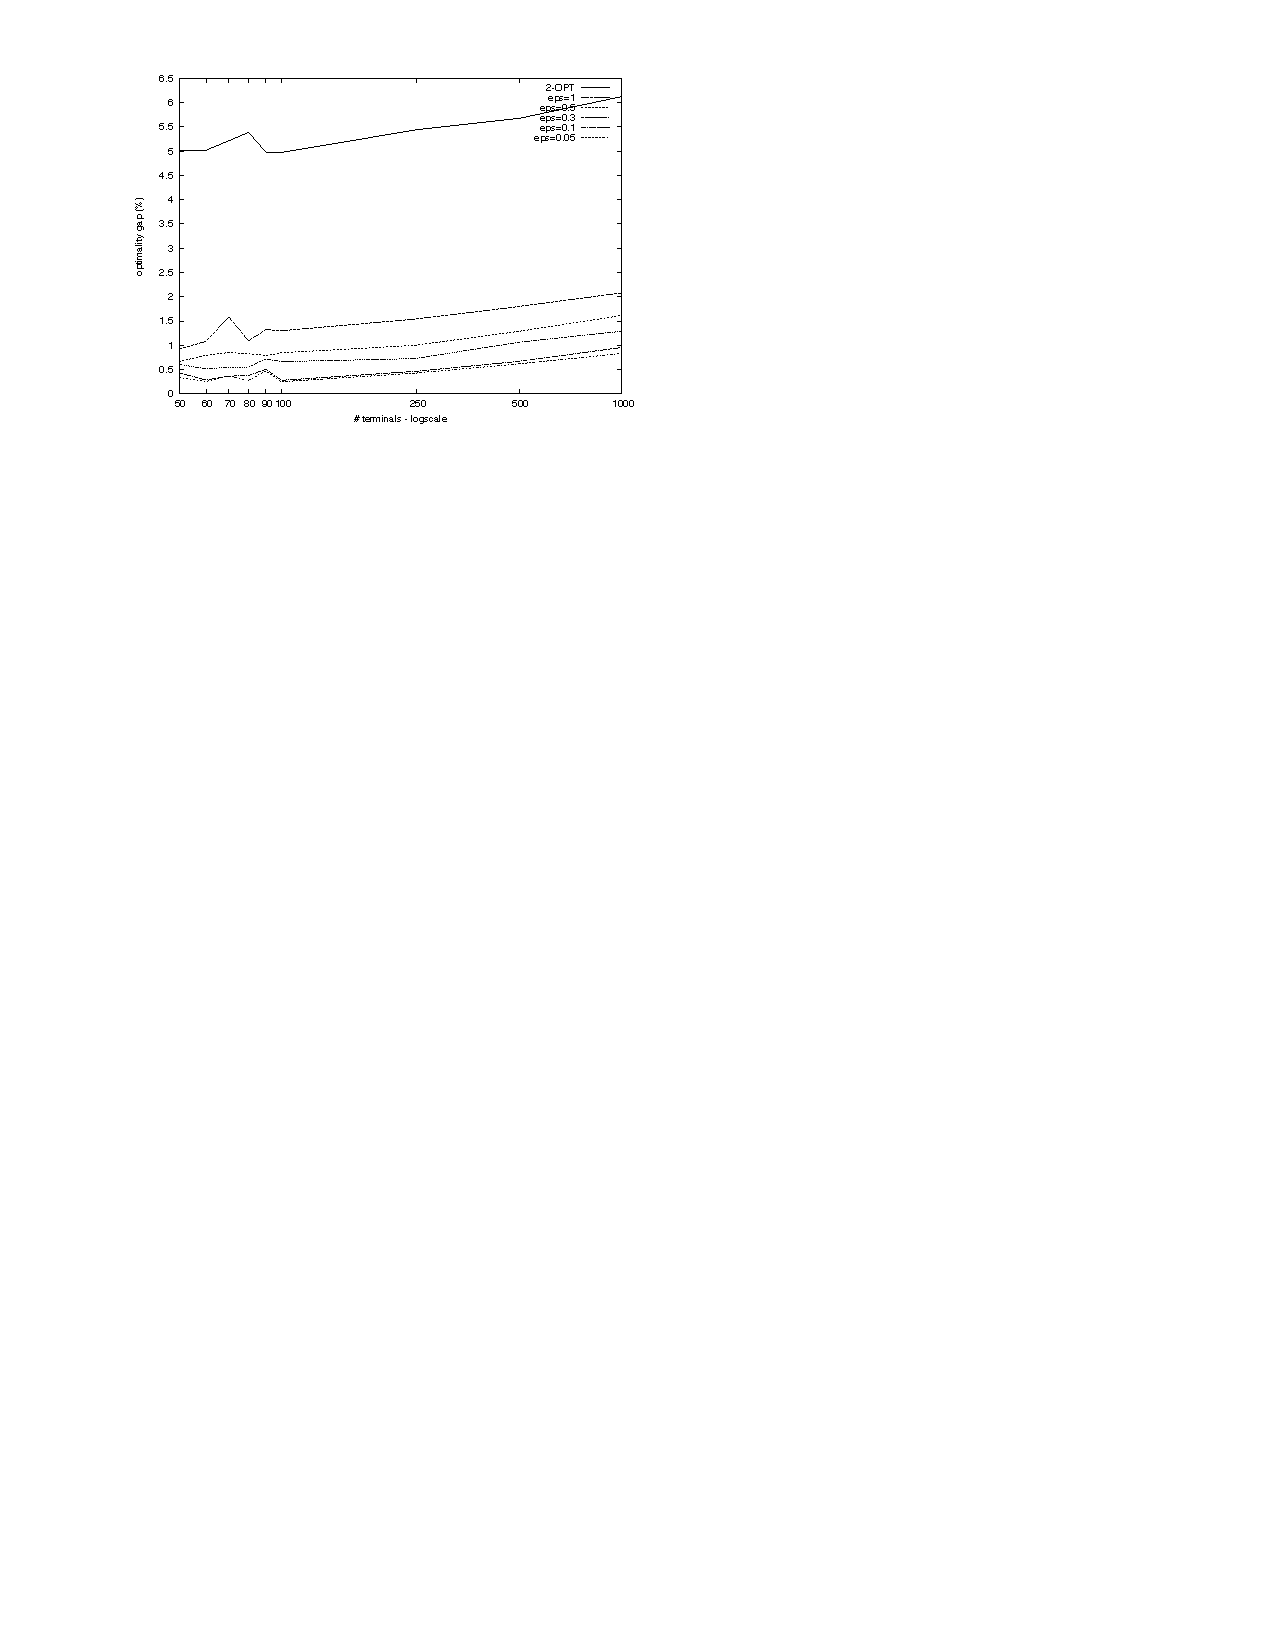
\includegraphics[scale=1.35]{imgs/experimento1.1.pdf}
%     \caption{Qualidade da solução nos experimentos para Árvore de Steiner. (\cite{TazariLargeConstants}).}
%     \label{fig:experiment1.1}
% \end{figure}

% \begin{figure}[h]
%     \centering
%     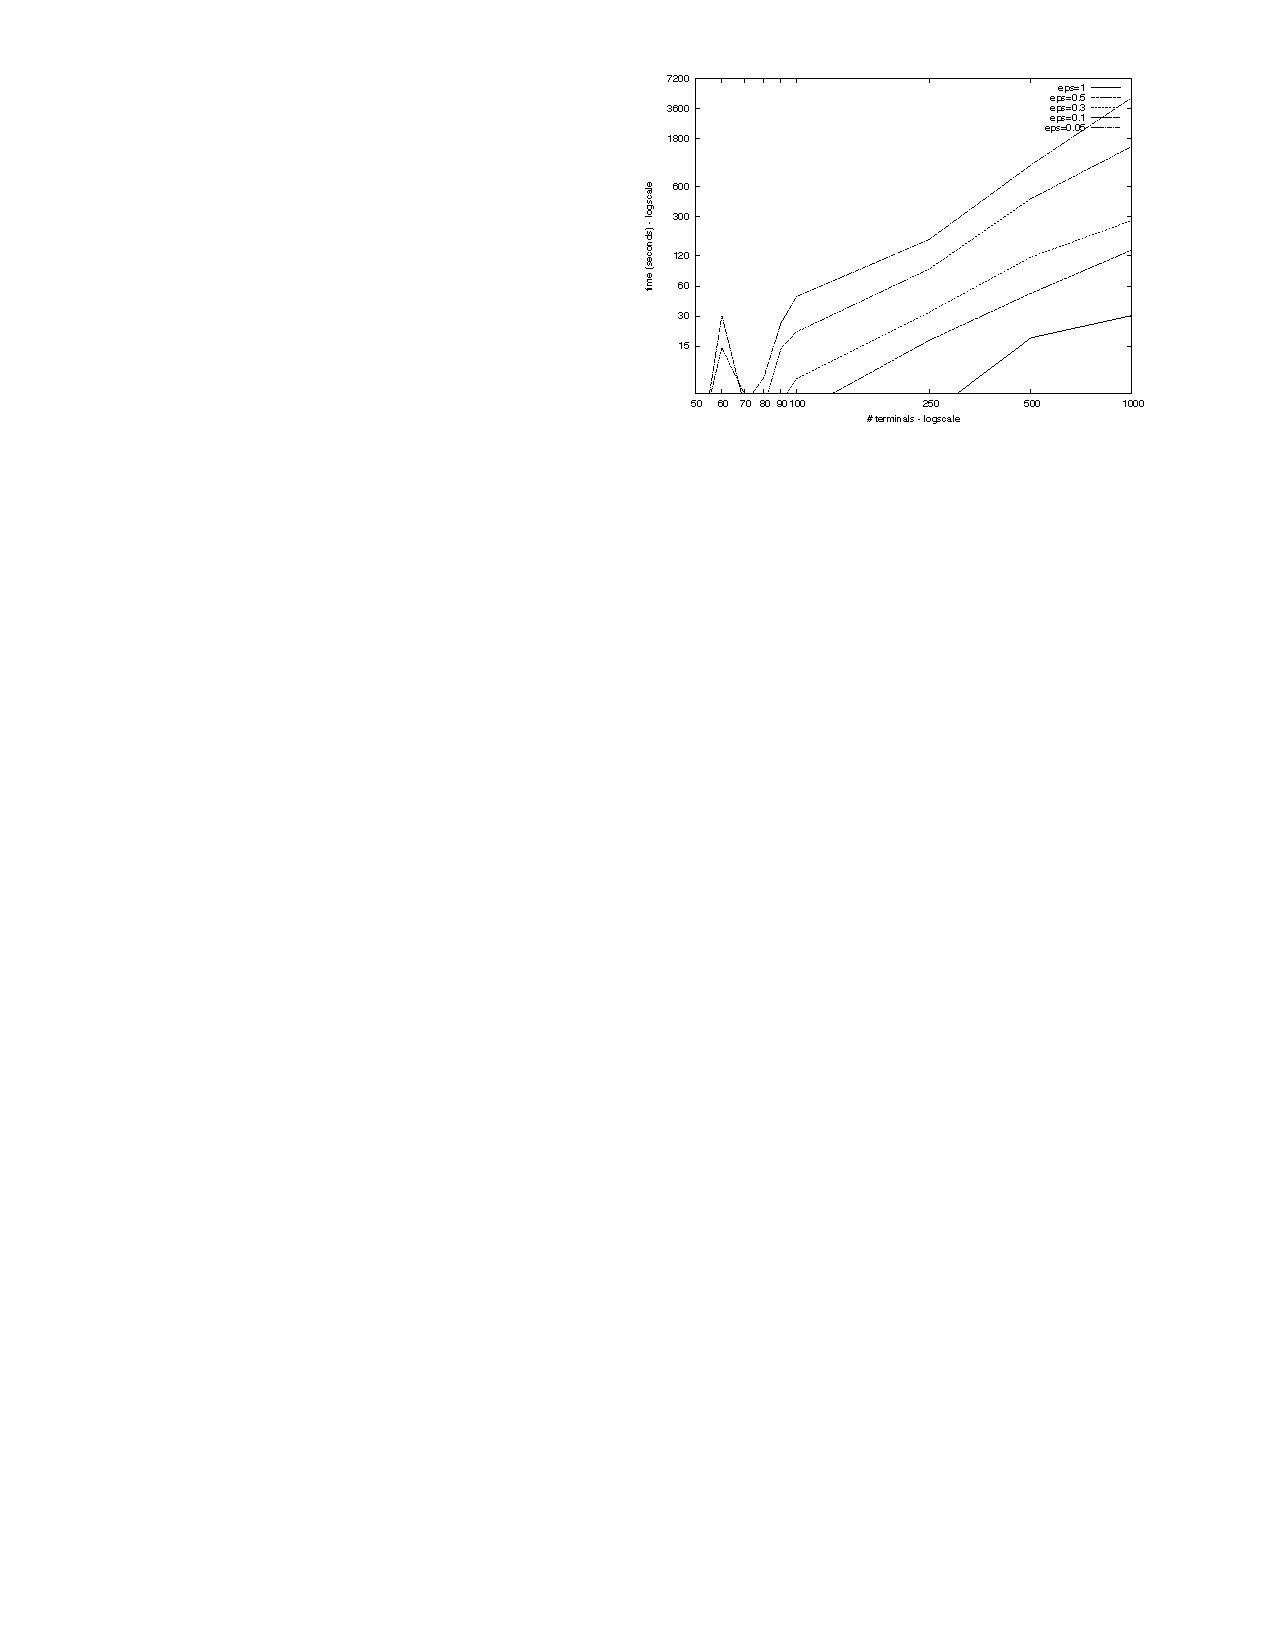
\includegraphics[scale=1.35]{imgs/experimento1.2.pdf}
%     \caption{Tempo de execução nos experimentos para Árvore de Steiner. (\cite{TazariLargeConstants}).}
%     \label{fig:experiment1.2}
% \end{figure}

% Nesse resultado é possível observar o claro \textit{trade-off} que existe entre qualdiade média da solução e o tempo de execução do algoritmo, dependendo do valor de \(\epsilon\). Em particular a qualidade obtida pelo PTAS foi bem superior ao do algoritmo de aproximação.

% Nessas mesmas instâncias, também foi testado a famosa heurística B1S (\cite{B1S}). Os resultados foram superiores a ambos o PTAS e o algoritmo aproximativo, obtendo em média um resultado 0,48\% próximo do ótimo em 9 segundos.

% Apesar do resultado muito positivo, o algoritmo B1S se mostra limitado em relação ao PTAS em instâncias arbitrariamente grandes. Em particular, os autores compararam ambos algoritmos em uma instância com 500 mil vértices obtendo resultados similares para ambos, mas com 1506 segundos de tempo de execução para o PTAS e 234758 segundos para a heurística.

In this work we intend to expand on the results found by \cite{LINTZMAYER2020134} by proposing a PTAS for the \(\steinercycle\) in graphs with bounded-genus. To do so we will use various techniques proposed by \cite{Bateni} and \cite{Borradaile2009b} for the Steiner Forest and Steiner Tree problems, respectively, such as the Mortar Graph, the Prize Collecting Clustering, and the spanner.

% Pretendemos extender o trabalho desenvolvido por \cite{LINTZMAYER2020134} propondo um PTAS para o \(\steinercycle\) em grafos com \textit{genus} limitado. Para alcançar esse objetivo, usaremos várias das técnicas propostas por \citeauthor{Bateni} e \citeauthor{Borradaile2009b} para os problemas de Floresta de Steiner e Árvore de Steiner, respectivamente. Além disso, de maneira similar ao que \cite{TazariLargeConstants} fizeram para Árvore de Steiner, planejamos realizar experimentos computacionais com instâncias do \(\steinercycle\), comparando implementações dos algoritmos testados por \citeauthor{Pereira2018TheSM} com o algoritmo que pretendemos desenvolver neste trabalho.